\documentclass[tikz]{standalone}
\usepackage{pgfplots}
\pgfplotsset{compat=1.15}
\usepackage{mathrsfs}
\usetikzlibrary{arrows,calc}
\usepackage{tkz-euclide}
\pagestyle{empty}

\definecolor{AngleClr}{rgb}{0,0.39215686274509803,0}
\definecolor{ShapeClr}{rgb}{0.6,0.2,0}

\begin{document}

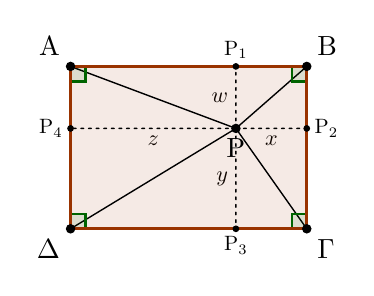
\begin{tikzpicture}[scale=.75]
\tkzSetUpLine[line width=1pt,color=black]
\tkzSetUpPoint[fill=black]

\tkzDefPoints{0/0/D,4/0/C,0/2.75/A,4/2.75/B,2/1.5/O,2.8/1.7/P}

\tkzDefPointBy[projection = onto A--B](P)\tkzGetPoint{P1}
\tkzDefPointBy[projection = onto B--C](P)\tkzGetPoint{P2}
\tkzDefPointBy[projection = onto C--D](P)\tkzGetPoint{P3}
\tkzDefPointBy[projection = onto D--A](P)\tkzGetPoint{P4}

\tkzLabelSegment[scale=0.8,left](P,P1){$w$}
\tkzLabelSegment[scale=0.8,below](P,P2){$x$}
\tkzLabelSegment[scale=0.8,left](P,P3){$y$}
\tkzLabelSegment[scale=0.8,below](P,P4){$z$}


\tkzFillPolygon[fill=ShapeClr,fill opacity=0.1,inner sep=1cm](A,B,C,D)

\tkzDrawSegments[line width=0.5pt,color=black](A,P B,P C,P D,P)
\tkzDrawSegments[line width=0.5pt,color=black,dashed,dash pattern=on 1pt off 1.75pt](P,P1 P,P2 P,P3 P,P4)

\tkzMarkRightAngles[line width=1pt, size=.25,color=AngleClr,fill=AngleClr,fill opacity=0.1](A,B,C B,C,D C,D,A D,A,B)

\tkzDrawPolygon[color=ShapeClr](A,B,C,D)
\tkzDrawPoints[size=3](A,B,C,D,P)
\tkzDrawPoints[size=2](P1,P2,P3,P4)
\tkzLabelPoint[above left](A){$\rm A$}
\tkzLabelPoint[above right](B){$\rm B$}
\tkzLabelPoint[below right](C){$\rm \Gamma$}
\tkzLabelPoint[below left](D){$\rm \Delta$}
\tkzLabelPoint[below](P){$\rm P$}

\tkzLabelPoint[scale=0.75,above](P1){${\rm P}_1$}
\tkzLabelPoint[scale=0.75,right](P2){${\rm P}_2$}
\tkzLabelPoint[scale=0.75,below](P3){${\rm P}_3$}
\tkzLabelPoint[scale=0.75,left](P4){${\rm P}_4$}

\end{tikzpicture}
\end{document}
